\chapter{Descrizione dell'applicativo}
    \section{Descrizione generale}
        L'applicativo denominato "SIRIUS" (Sistema Informativo Relazionale Integrato per l'Umane Risorse) permette la gestione di un database per la gestione di personale, laboratori e progetti all'interno dell'azienda. Attraverso diverse sezioni è possibile mostrare i dati relativi a quella sezione nel database. E' anche possibile aggiungere, modificare ed eliminare dati dal database.

    \section{Frames Home}
        Nella finestra "Home" l'utente può decidere a quale area accedere da cui poi effettuare le operazioni abilitate per quell'area.
        \begin{figure}[htbp!]
            \centering
                \vspace{2\baselineskip}
                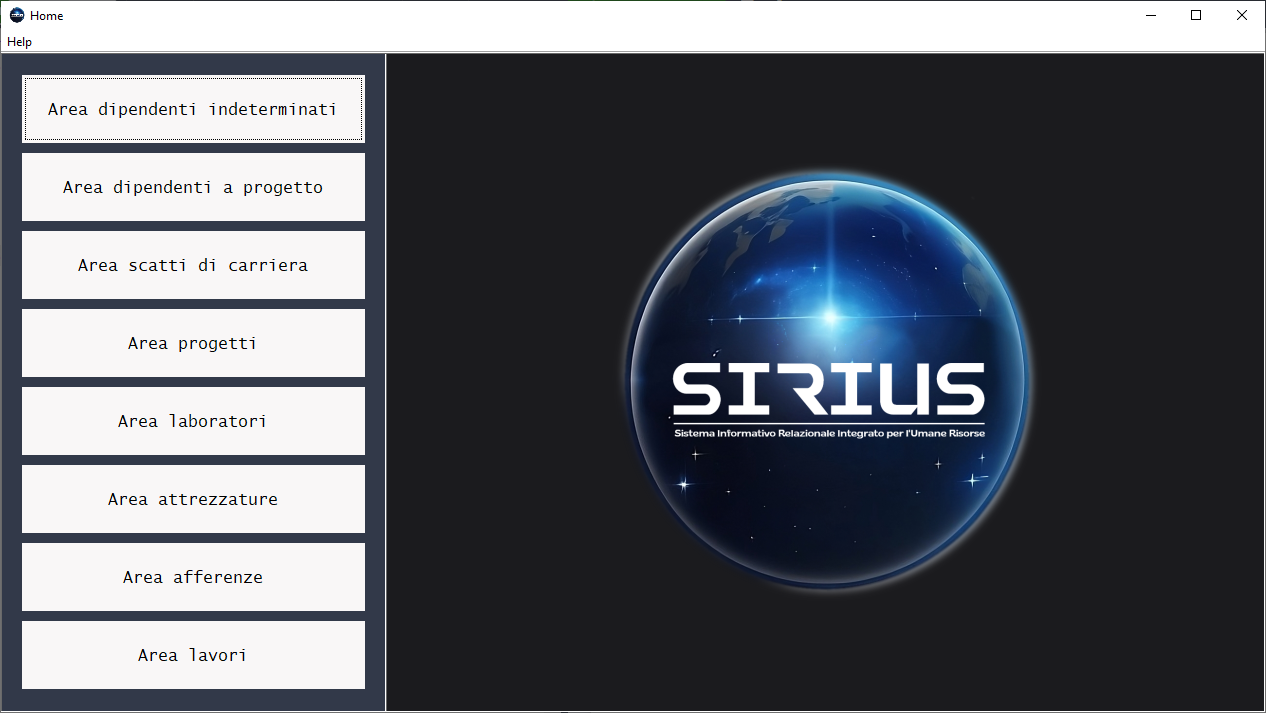
\includegraphics[width=0.9\linewidth]{Immagini/Frames/Frame Home.png}
            \caption{Frame Home}
            \label{fig:Frame Home}
        \end{figure}

    \newpage

    \section{Frames Dipendenti indeterminati}
        \subsection {Finestra "Area dipendenti indeterminati"}
            Nella finestra "Area dipendenti indeterminati" l'utente avrà a disposizione una tabella con tutti i dati nel database relativi ai dipendenti assunti a tempo indeterminato. Ogni colonna può essere ordinata in senso crescente o decrescente.\\
            Da qui, attraverso i bottoni in basso, si potrà decidere se tornare alla schermata home (indietro), aggiungere un nuovo dipendente a tempo indeterminato (aggiungi) o selezionare un dipendente e modificarne i dati (modifica). Cliccando su "aggiungi" o "modifica" si aprirà la finestra "aggiungi/modifica Dipendenti indeterminati". Dato che si intende tenere traccia di tutti i dipendenti a tempo indeterminato, non è possibile eliminarne alcuno dall'applicativo.\\
            In alto è inoltre presente una barra di ricerca. I valori inseriti al suo interno saranno cercati tra tutti i campi della tabella.
            \begin{figure}[htbp!]
                \centering
                    \vspace{2\baselineskip}
                    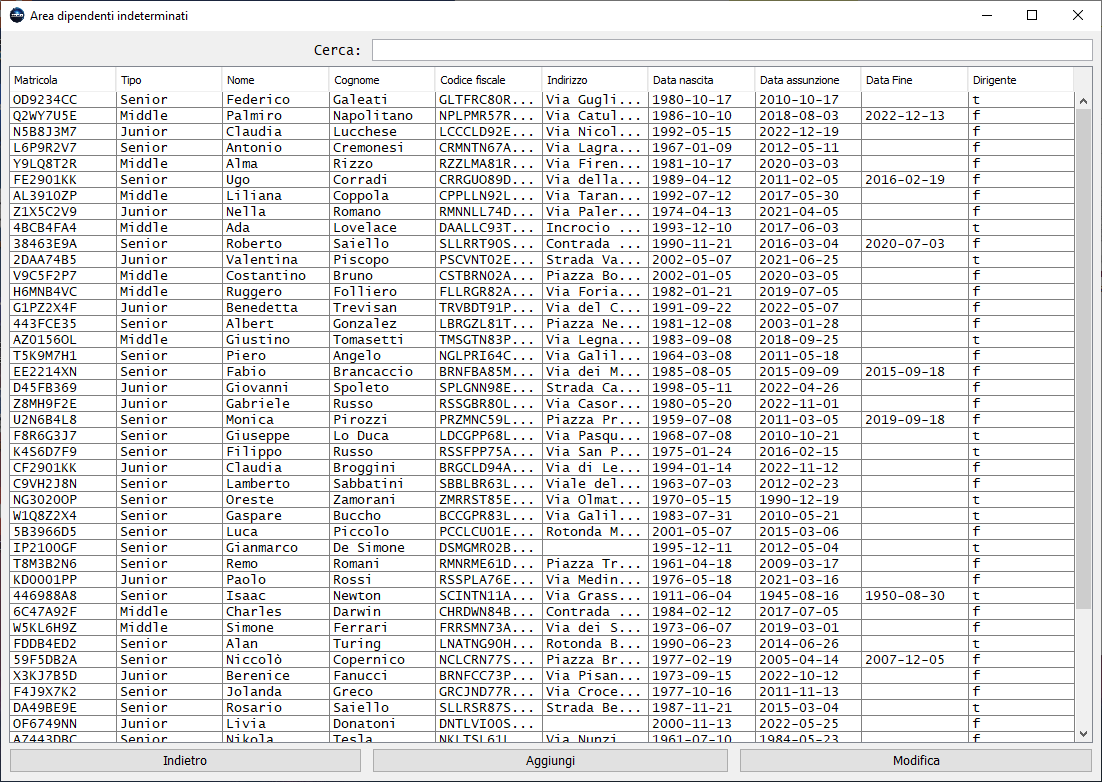
\includegraphics[width=0.9\linewidth]{Immagini/Frames/Frame Area/Frame Area dipendenti indeterminati.png}
                \caption{Frame Area dipendenti indeterminati}
                \label{fig:Frame Area dipendenti indeterminati}
            \end{figure}

    \newpage

        \subsection {Finestra "aggiungi/modifica Dipendenti indeterminati"}
            Nella finestra "aggiungi/modifica Dipendenti indeterminati" l'utente potrà inserire i valori negli appositi campi per aggiungere un dipendente al database. In particolare, potrà inserire nome, cognome, codice fiscale, matricola, tipo dipendente (e spuntare la relativa checkbox se si intende aggiungere un dirigente), indirizzo (il campo sarà abilitato spuntando la relativa checkbox), data di nascita, data di assunzione (spuntando la relativa checkbox il campo verrà automaticamente compilato con la data odierna) e la data di fine rapporto (spuntando la prima checkbox si rende disponibile il campo, mentre con la seconda checkbox si compila automaticamente con la data odierna).\\
            Con i bottoni in basso si può annullare o confermare l'aggiunta.\\
            Se, invece, nella finestra "Area dipendente indeterminato" si è cliccati su "modifica", i campi verranno precompilati con quelli del dipendente selezionato. Dopodichè si potrà procedere con la modifica.
            \begin{figure}[htbp!]
                \centering
                    \vspace{2\baselineskip}
                    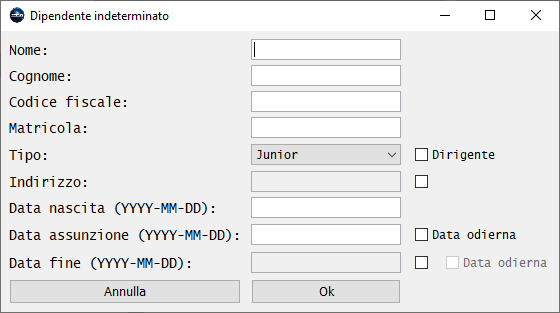
\includegraphics[width=0.6\linewidth]{Immagini/Frames/Frame aggiungi-modifica/Frame Dipendente indeterminato aggiungi-modifica.png}
                \caption{Frame Dipendente indeterminato aggiungi-modifica}
                \label{fig:Frame Dipendente indeterminato aggiungi-modifica}
            \end{figure}

    \newpage

    \section{Frames Dipendenti a progetto}
        \subsection {Finestra "Area dipendenti progetto"}
            Nella finestra "Area dipendenti progetto" l'utente avrà a disposizione una tabella con tutti i dati nel database relativi ai dipendenti assunti con contratto a progetto. Ogni colonna può essere ordinata in senso crescente o decrescente.\\
            Da qui, attraverso i bottoni in basso, si potrà decidere se tornare alla schermata home (indietro), aggiungere un nuovo dipendente a tempo a progetto (aggiungi) o selezionare un dipendente e modificarne i dati (modifica). Cliccando su "aggiungi" o "modifica" si aprirà la finestra "aggiungi/modifica Dipendenti progetto". Dato che si intende tenere traccia di tutti i dipendenti con contratto a progetto, non è possibile eliminarne alcuno dall'applicativo.\\
            In alto è inoltre presente una barra di ricerca. I valori inseriti al suo interno saranno cercati tra tutti i campi della tabella.
            \begin{figure}[htbp!]
                \centering
                    \vspace{2\baselineskip}
                    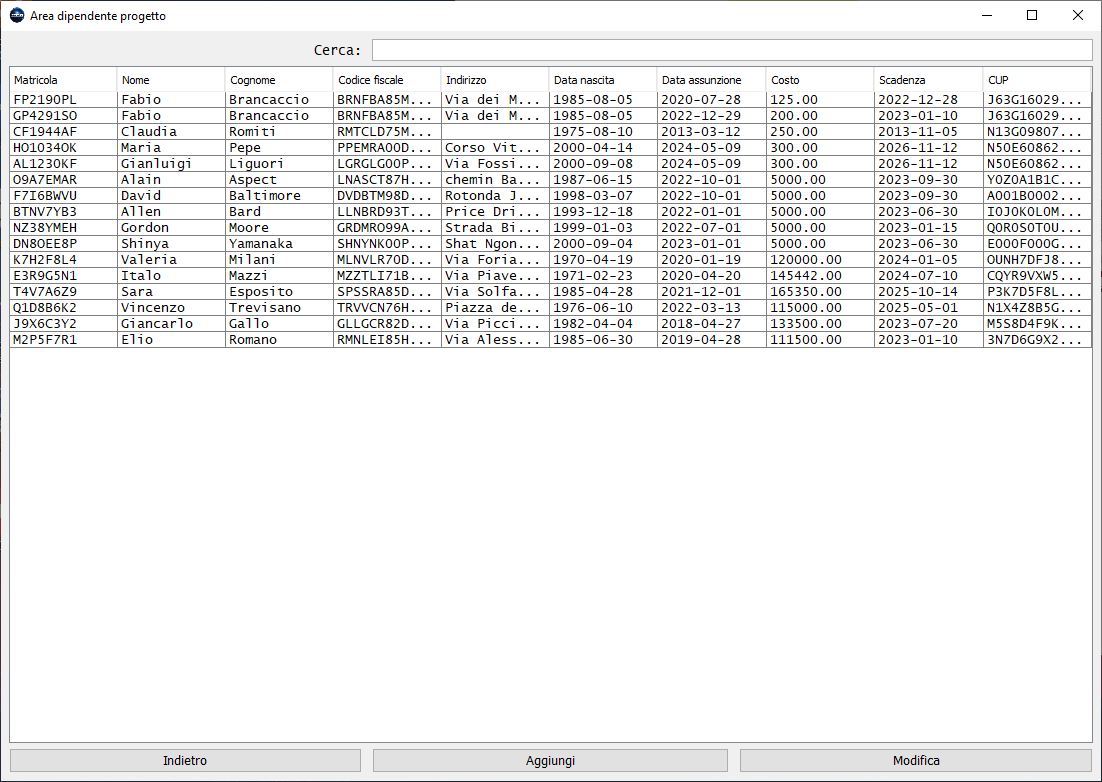
\includegraphics[width=0.9\linewidth]{Immagini/Frames/Frame Area/Frame Area dipendente progetto.png}
                \caption{Frame Area dipendenti progetto}
                \label{fig:Frame Area dipendenti progetto}
            \end{figure}

    \newpage

        \subsection {Finestra "aggiungi/modifica Dipendenti progetto"}
            Nella finestra "aggiungi/modifica Dipendenti progetto" l'utente potrà inserire i valori negli appositi campi per aggiungere un dipendente al database. In particolare, potrà inserire nome, cognome, codice fiscale, matricola, indirizzo (il campo sarà abilitato spuntando la relativa checkbox), data di nascita, data di assunzione (spuntando la relativa checkbox il campo verrà automaticamente compilato con la data odierna), la data di scadenza del contratto (spuntando la checkbox si compila automaticamente con la data odierna), il costo del contratto a progetto e quale progetto ha ingaggiato il dipendente che stiamo inserendo.\\
            Con i bottoni in basso si può annullare o confermare l'aggiunta.\\
            Se, invece, nella finestra "Area dipendente progetto" si è cliccati su "modifica", i campi verranno precompilati con quelli del dipendente selezionato. Dopodichè si potrà procedere con la modifica.
            \begin{figure}[htbp!]
                \centering
                    \vspace{2\baselineskip}
                    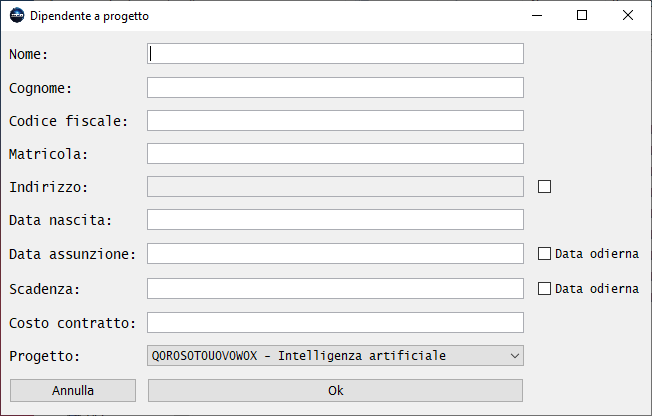
\includegraphics[width=0.6\linewidth]{Immagini/Frames/Frame aggiungi-modifica/Frame Dipendente a progetto aggiungi-modifica.png}
                \caption{Frame Dipendente a progetto aggiungi-modifica}
                \label{fig:Frame Dipendente a progetto aggiungi-modifica}
            \end{figure}

    \newpage

    \section{Frames Scatti di carriera}
        \subsection {Finestra "Area scatti di carriera"}
            Nella finestra "Area scatti di carriera" l'utente avrà a disposizione una tabella con tutti i dati nel database relativi agli scatti di carriera. Ogni colonna può essere ordinata in senso crescente o decrescente.\\
            Da qui, attraverso i bottoni in basso, si potrà decidere se tornare alla schermata home (indietro), aggiungere un nuovo scatti di carriera (aggiungi) o selezionare uno scatti di carriera di tipo dirigenziale e modificarne i dati (modifica). Cliccando su "aggiungi" o "modifica" si aprirà la finestra "aggiungi/modifica Dipendenti progetto". Dato che si intende tenere traccia di tutti gli scatti di carriera, non è possibile eliminarne alcuno tramite app. Inoltre, gli scatti di carriera di tipo "Middle" e "Senior" sono automaticamente gestiti dall'applicativo.\\
            In alto è inoltre presente una barra di ricerca. I valori inseriti al suo interno saranno cercati tra tutti i campi della tabella.
            \begin{figure}[htbp!]
                \centering
                    \vspace{2\baselineskip}
                    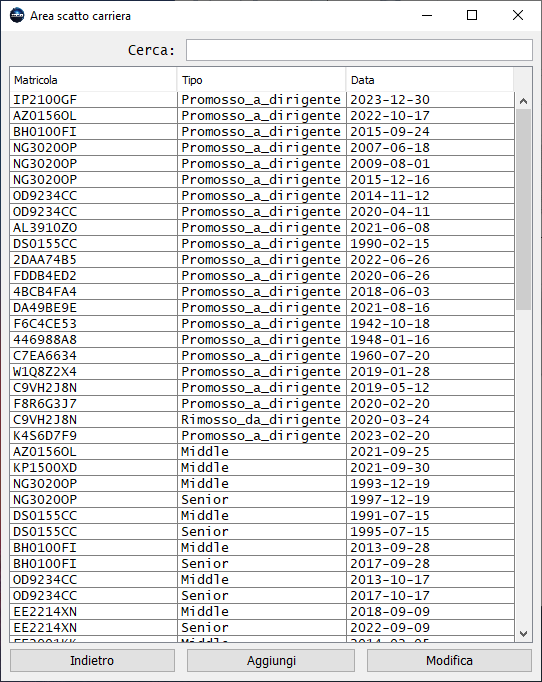
\includegraphics[width=0.6\linewidth]{Immagini/Frames/Frame Area/Frame Area scatto carriera.png}
                \caption{Frame Area scatto carriera}
                \label{fig:Frame Area scatto carriera}
            \end{figure}

    \newpage

        \subsection {Finestra "aggiungi/modifica Scatto carriera"}
            Nella finestra "aggiungi/modifica Scatto carriera" l'utente potrà inserire i valori negli appositi campi per aggiungere uno scatto di carriera al database. In particolare, potrà inserire il dipendente che effettua lo scatto, la data in cui viene effettuato (spuntando la relativa checkbox il campo verrà automaticamente compilato con la data odierna) e il tipo di scatto (gli scatti di tipo "Middle" e "Senior" sono automaticamente gestiti dall'applicativo). Per confermare il tipo di scatto è necessario cliccare su "Seleziona".\\
            Con i bottoni in basso si può annullare o confermare l'aggiunta.\\
            Se, invece, nella finestra "Area scatto carriera" si è cliccati su "modifica", i campi verranno precompilati con quelli dello scatto di carriera selezionato. Dopodichè si potrà procedere con la modifica.
            \begin{figure}[htbp!]
                \centering
                    \vspace{2\baselineskip}
                    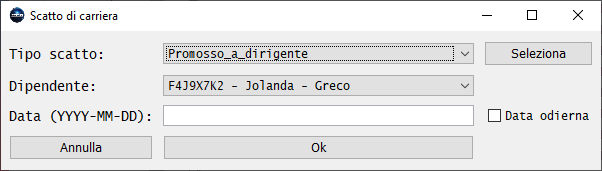
\includegraphics[width=0.7\linewidth]{Immagini/Frames/Frame aggiungi-modifica/Frame Scatto di carriera aggiungi-modifica.png}
                \caption{Frame Scatto carriera aggiungi-modifica}
                \label{fig:Frame Scatto carriera aggiungi-modifica}
            \end{figure}

    \newpage

    \section{Frames Progetto}
        \subsection {Finestra "Area progetto"}
            Nella finestra "Area progetto" l'utente avrà a disposizione una tabella con tutti i dati nel database relativi ai progetti. Ogni colonna può essere ordinata in senso crescente o decrescente.\\
            Da qui, attraverso i bottoni in basso, si potrà decidere se tornare alla schermata home (indietro), aggiungere un nuovo progetto (aggiungi) o selezionare un progetto e modificarne i dati (modifica). Cliccando su "aggiungi" o "modifica" si aprirà la finestra "aggiungi/modifica Progetto". Dato che si intende tenere traccia di tutti i progetti, non è possibile eliminarne alcuno tramite app.\\
            In alto è inoltre presente una barra di ricerca. I valori inseriti al suo interno saranno cercati tra tutti i campi della tabella.
            \begin{figure}[htbp!]
                \centering
                    \vspace{2\baselineskip}
                    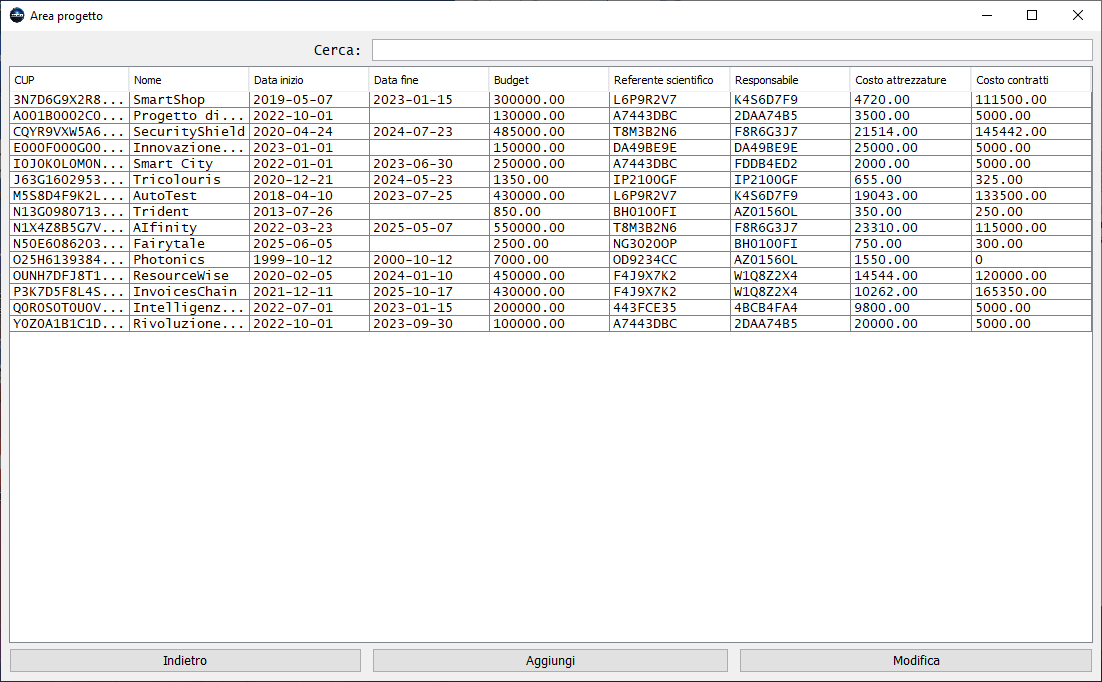
\includegraphics[width=0.9\linewidth]{Immagini/Frames/Frame Area/Frame Area progetto.png}
                \caption{Frame Area progetto}
                \label{fig:Frame Area progetto}
            \end{figure}

    \newpage

        \subsection {Finestra "aggiungi/modifica Progetto"}
            Nella finestra "aggiungi/modifica Progetto" l'utente potrà inserire i valori negli appositi campi per aggiungere un progetto al database. In particolare, potrà inserire il nome, il CUP, il budget istanziato per il progetto, la data di inizio progetto, la data di fine progetto (Si può rendere disponibile il campo spuntando la prima checkbox, confermare la data inserita cliccando su "Seleziona" e spuntare la seconda checkbox per precompilare il campo con la data odierna), il referente scientifico e il responsabile.\\
            Con i bottoni in basso si può annullare o confermare l'aggiunta.\\
            Se, invece, nella finestra "Area progetto" si è cliccati su "modifica", i campi verranno precompilati con quelli del progetto selezionato. Dopodichè si potrà procedere con la modifica.
            \begin{figure}[htbp!]
                \centering
                    \vspace{2\baselineskip}
                    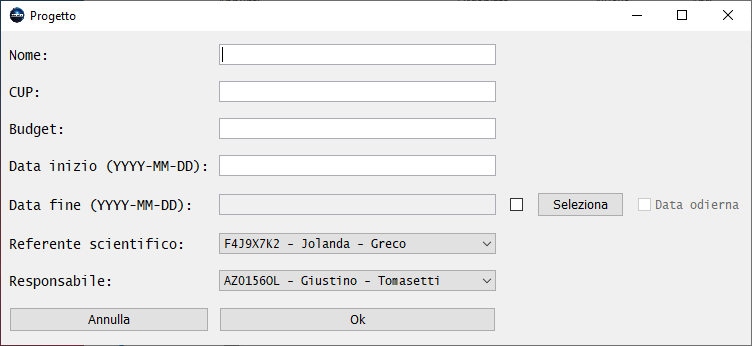
\includegraphics[width=0.7\linewidth]{Immagini/Frames/Frame aggiungi-modifica/Frame Progetto aggiungi-modifica.png}
                \caption{Frame Progetto aggiungi-modifica}
                \label{fig:Frame Progetto aggiungi-modifica}
            \end{figure}

    \newpage

    \section{Frames Laboratorio}
        \subsection {Finestra "Area laboratorio"}
            Nella finestra "Area laboratorio" l'utente avrà a disposizione una tabella con tutti i dati nel database relativi ai laboratori. Ogni colonna può essere ordinata in senso crescente o decrescente.\\
            Da qui, attraverso i bottoni in basso, si potrà decidere se tornare alla schermata home (indietro), aggiungere un nuovo laboratorio (aggiungi), selezionare un laboratorio e modificarne i dati (modifica) o eliminare il laboratorio selezionato. Cliccando su "aggiungi" o "modifica" si aprirà la finestra "aggiungi/modifica Laboratorio".\\
            In alto è inoltre presente una barra di ricerca. I valori inseriti al suo interno saranno cercati tra tutti i campi della tabella.
            \begin{figure}[htbp!]
                \centering
                    \vspace{2\baselineskip}
                    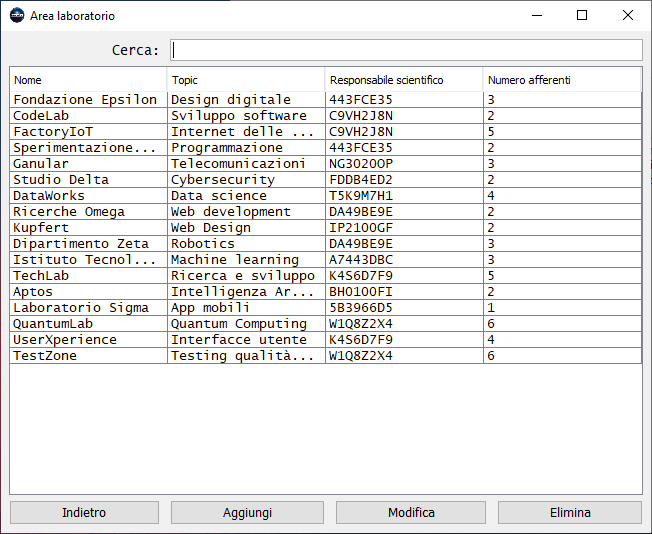
\includegraphics[width=0.9\linewidth]{Immagini/Frames/Frame Area/Frame Area laboratorio.png}
                \caption{Frame Area laboratorio}
                \label{fig:Frame Area laboratorio}
            \end{figure}

    \newpage

        \subsection {Finestra "aggiungi/modifica Laboratorio"}
            Nella finestra "aggiungi/modifica Laboratorio" l'utente potrà inserire i valori negli appositi campi per aggiungere un laboratorio al database. In particolare, potrà inserire il nome, il topic e il responsabile scientifico.\\
            Con i bottoni in basso si può annullare o confermare l'aggiunta.\\
            Se, invece, nella finestra "Area laboratorio" si è cliccati su "modifica", i campi verranno precompilati con quelli del laboratorio selezionato. Dopodichè si potrà procedere con la modifica.
            \begin{figure}[htbp!]
                \centering
                    \vspace{2\baselineskip}
                    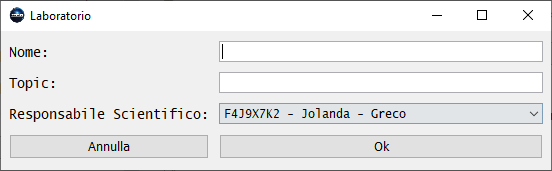
\includegraphics[width=0.7\linewidth]{Immagini/Frames/Frame aggiungi-modifica/Frame Laboratorio aggiungi-modifica.png}
                \caption{Frame Laboratorio aggiungi-modifica}
                \label{fig:Frame Laboratorio aggiungi-modifica}
            \end{figure}

    \newpage

    \section{Frames Attrezzatura}
        \subsection {Finestra "Area attrezzatura"}
            Nella finestra "Area attrezzatura" l'utente avrà a disposizione una tabella con tutti i dati nel database relativi alle attrezzature. Ogni colonna può essere ordinata in senso crescente o decrescente.\\
            Da qui, attraverso i bottoni in basso, si potrà decidere se tornare alla schermata home (indietro), aggiungere una nuova attrezzatura (aggiungi) o selezionare un'attrezzatura e modificarne i dati (modifica). Cliccando su "aggiungi" o "modifica" si aprirà la finestra "aggiungi/modifica Attrezzatura". Dato che si intende tenere traccia di tutte le attrezzature, non è possibile eliminarne alcuna tramite app.\\
            In alto è inoltre presente una barra di ricerca. I valori inseriti al suo interno saranno cercati tra tutti i campi della tabella.
            \begin{figure}[htbp!]
                \centering
                    \vspace{2\baselineskip}
                    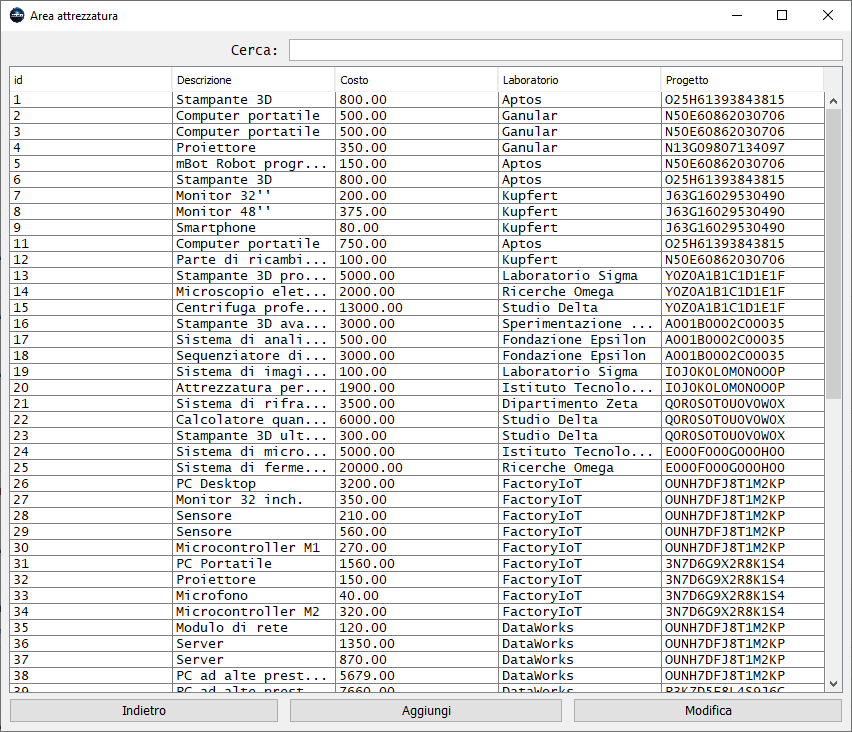
\includegraphics[width=0.9\linewidth]{Immagini/Frames/Frame Area/Frame Area attrezzatura.png}
                \caption{Frame Area attrezzatura}
                \label{fig:Frame Area attrezzatura}
            \end{figure}

    \newpage

        \subsection {Finestra "aggiungi/modifica Attrezzatura"}
            Nella finestra "aggiungi/modifica Attrezzatura" l'utente potrà inserire i valori negli appositi campi per aggiungere un'attrezzatura al database. In particolare, potrà inserire la descrizione, il costo, il progetto che ha acquistato l'attrezzatura (una volta scelto, è necessario confermare cliccando su "Seleziona") e il laboratorio a è stata assegnata, se esiste (il campo può essere abilitato tramite l'apposita checkbox)\\
            Con i bottoni in basso si può annullare o confermare l'aggiunta.\\
            Se, invece, nella finestra "Area attrezzatura" si è cliccati su "modifica", i campi verranno precompilati con quelli del laboratorio selezionato. Dopodichè si potrà procedere con la modifica.
            \begin{figure}[htbp!]
                \centering
                    \vspace{2\baselineskip}
                    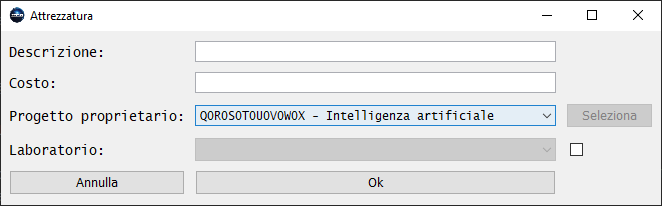
\includegraphics[width=0.7\linewidth]{Immagini/Frames/Frame aggiungi-modifica/Frame Attrezzatura aggiungi-modifica.png}
                \caption{Frame Attrezzatura aggiungi-modifica}
                \label{fig:Frame Attrezzatura aggiungi-modifica}
            \end{figure}

    \newpage

    \section{Frames Afferenze}
        \subsection {Finestra "Area afferenze"}
            Nella finestra "Area afferenze" l'utente avrà a disposizione una tabella con tutti i dati nel database relativi alle afferenze ai laboratori. Ogni colonna può essere ordinata in senso crescente o decrescente.\\
            Da qui, attraverso i bottoni in basso, si potrà decidere se tornare alla schermata home (indietro), aggiungere una nuova afferenza (aggiungi), selezionare un'afferenza e modificarne i dati (modifica) o eliminare l'afferenza selezionata. Cliccando su "aggiungi" o "modifica" si aprirà la finestra "aggiungi/modifica Afferenza".\\
            In alto è inoltre presente una barra di ricerca. I valori inseriti al suo interno saranno cercati tra tutti i campi della tabella.
            \begin{figure}[htbp!]
                \centering
                    \vspace{2\baselineskip}
                    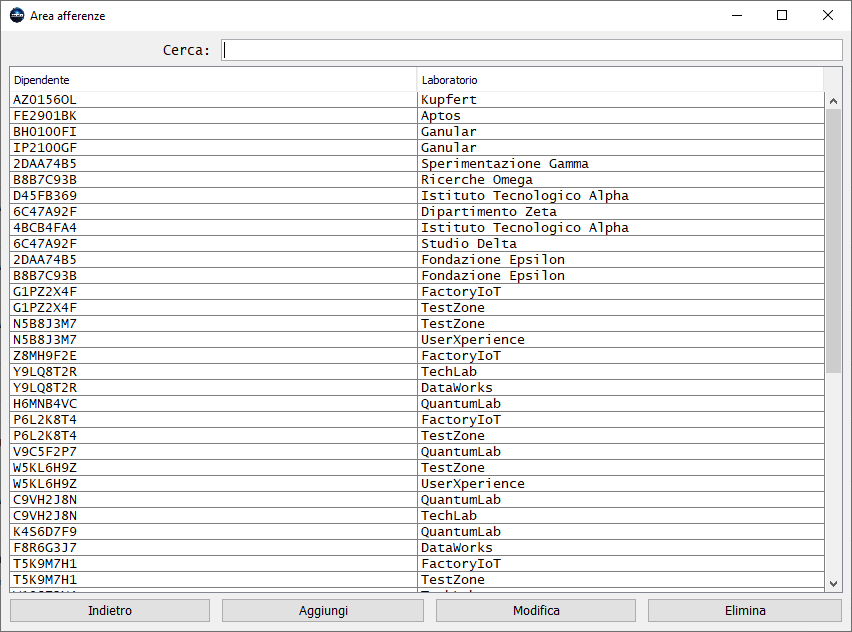
\includegraphics[width=0.9\linewidth]{Immagini/Frames/Frame Area/Frame Area afferenze.png}
                \caption{Frame Area afferenze}
                \label{fig:Frame Area afferenze}
            \end{figure}

    \newpage

        \subsection {Finestra "aggiungi/modifica Afferenza"}
            Nella finestra "aggiungi/modifica Afferenza" l'utente potrà inserire i valori negli appositi campi per aggiungere un'afferenza al database. In particolare, potrà inserire il dipendente e il laboratorio a cui afferisce.\\
            Con i bottoni in basso si può annullare o confermare l'aggiunta.\\
            Se, invece, nella finestra "Area afferenza" si è cliccati su "modifica", i campi verranno precompilati con quelli dell'afferenza selezionata. Dopodichè si potrà procedere con la modifica.
            \begin{figure}[htbp!]
                \centering
                    \vspace{2\baselineskip}
                    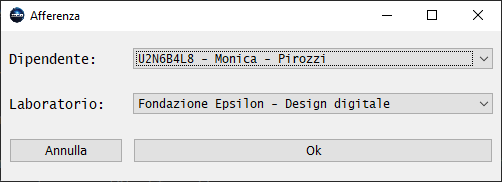
\includegraphics[width=0.7\linewidth]{Immagini/Frames/Frame aggiungi-modifica/Frame Afferenza aggiungi-modifica.png}
                \caption{Frame Afferenza aggiungi-modifica}
                \label{fig:Frame Afferenza aggiungi-modifica}
            \end{figure}

    \newpage

    \section{Frames Lavorare}
        \subsection {Finestra "Area lavorare"}
            Nella finestra "Area lavorare" l'utente avrà a disposizione una tabella con tutti i dati nel database relativi alle associazioni di "lavorare" tra laboratori e progetti. Ogni colonna può essere ordinata in senso crescente o decrescente.\\
            Da qui, attraverso i bottoni in basso, si potrà decidere se tornare alla schermata home (indietro), aggiungere un nuovo lavoro (aggiungi), selezionare un lavoro e modificarne i dati (modifica) o eliminare il lavoro selezionato. Cliccando su "aggiungi" o "modifica" si aprirà la finestra "aggiungi/modifica Lavorare".\\
            In alto è inoltre presente una barra di ricerca. I valori inseriti al suo interno saranno cercati tra tutti i campi della tabella.
            \begin{figure}[htbp!]
                \centering
                    \vspace{2\baselineskip}
                    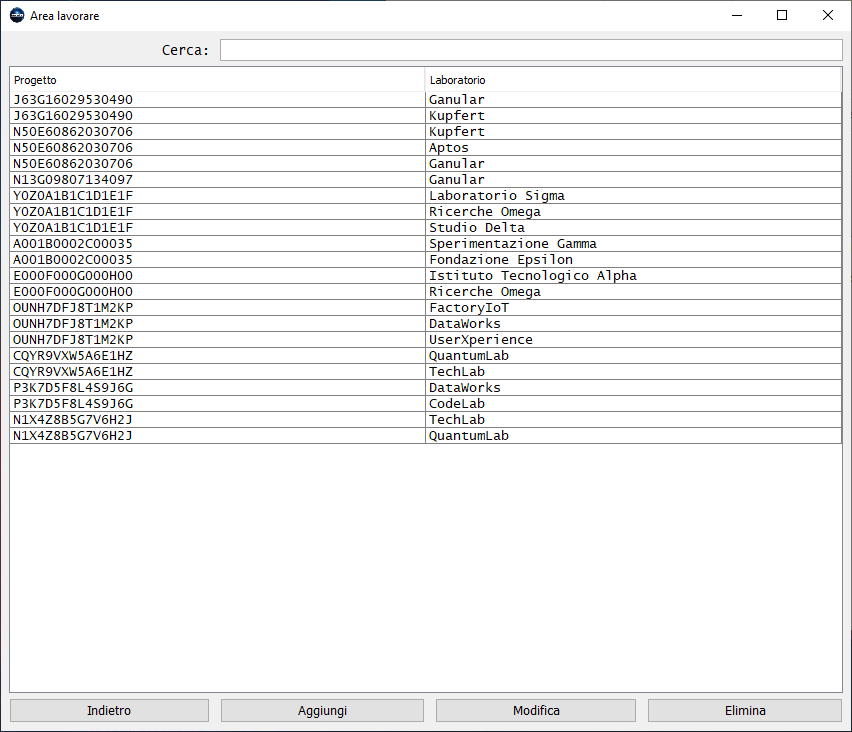
\includegraphics[width=0.9\linewidth]{Immagini/Frames/Frame Area/Frame Area lavorare.png}
                \caption{Frame Area lavorare}
                \label{fig:Frame Area lavorare}
            \end{figure}

    \newpage

        \subsection {Finestra "aggiungi/modifica Lavorare"}
            Nella finestra "aggiungi/modifica Lavori" l'utente potrà inserire i valori negli appositi campi per aggiungere un'associazione di lavoro tra laboratorio e progetto al database. In particolare, potrà inserire il progetto e il laboratorio che ci lavora.\\
            Con i bottoni in basso si può annullare o confermare l'aggiunta.\\
            Se, invece, nella finestra "Area lavorare" si è cliccati su "modifica", i campi verranno precompilati con quelli del laboratorio selezionato. Dopodichè si potrà procedere con la modifica.
            \begin{figure}[htbp!]
                \centering
                    \vspace{2\baselineskip}
                    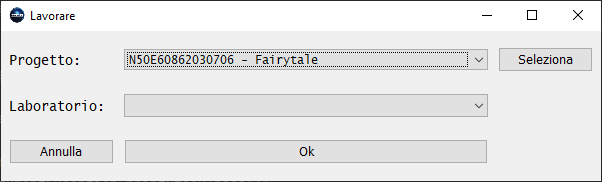
\includegraphics[width=0.7\linewidth]{Immagini/Frames/Frame aggiungi-modifica/Frame Lavorare aggiungi-modifica.png}
                \caption{Frame Lavorare aggiungi-modifica}
                \label{fig:Frame Lavorare aggiungi-modifica}
            \end{figure}